\chapter{Umsetzung} \label{sec:Umsetzung}

\section{Architektur}
Auf Basis der Grundlagen und Analyse wird die Architektur des Systems erstellt.
In der Architektur werden alle wichtigen Entscheidungen, welche für die
Entwicklung des Systems relevant und von technischer Natur sind, berücksichtigt. Die Architektur dient als Grundlage für die darauffolgende Umsetzung.

\section{Raspberry Pi}

\subsection{Sensoren}
\begin{itemize}
	\item Kameramodul
	\item Temperatursensor
	\item Luftfeuchtigkeitssensor
	\item Luftqualitätssensor 
\end{itemize}


\subsection{Sensor Adapter}
Der Sensor Adapter ist notwendig, um die Daten aus den Sensoren auszulesen und anschließen abzuspeichern. Nachfolgend soll erklärt werden, wie die Sensoren verschaltet sein müssen, damit Eingangssignale ausgewertet werden können. 

\subsubsection{Fester/ Tür-Status}
Der Aufbau um eine Tür 

\subsection{Persistenter Speicher}
Basierend auf den Grundlagen soll eine relationale Datenbank zum Speichern der Sensorwerte genutzt werden. Dabei muss die Datenbank kompatibel mit dem Raspberry Pi sein, sowie möglichst ressourcenschonend agieren. \\Es ist nicht notwendig Daten über das Netzwerk in die Tabelle einzutragen, da alle Sensoren über den Raspberry eingelesen werden können und die Datenbank somit nur lokal verfügbar sein muss.  

Anforderungen:\\
-Lokal \\
-Schreibzugriffe über das Netzwerk\\
-Concurrent writers?\\
-Big Data -> wir haben nur kleine Datenmengen\\
-Embedded\\
-Small / Hardwareressourcen/ leichtgewichtig\\
-Portabilität\\
-User Management -> nicht notwendig\\
-Kompatibilität mit Raspberry\\

Daten nur speichern und nach außen verfügbar machen.

Vergleich in Datei schreiben, MySQL, SQLite\\
.
\subsubsection{SQLite}
Die SQLite Datenbank bietet für unsere definierten Einsatzzweck ausreichende Funktionalität an. Die Anwendung ist leichtgewichtig und läuft lokal. Außerdem verfolgt die Datenbank bei Transaktionen das ACID (atomic, consistent, isolated, durable) Prinzip. Datenbankzugriffe geschehen mit SQL. Alle Datenbanktabellen sind lokal in einer Datenbank-Datei gespeichert. Dies kann somit einfach kopiert werden, falls ein neuer Raspberry zum Einsatz kommen sollte.\\
Da jeder Raspberry seine eigene Datenbank besitzen sollte, damit keine privaten Daten zentral auf einer Datenbank abgelegt werden eignet sich SQLite ebenfalls gut. 
*******
https://www.sqlite.org/features.html

hat keine Server prozess, zero-configuration, trasaction SQL, read writes directly into ordinary disk file
single disk file 
ACID
Full featured SQL
cross platform
standalone command line interface

content BLOB -> Dokument kann in db abgelegt werden


\subsection{Datenbankschema}

\subsection{Flows Node-Red}
\begin{figure}
	\centering
	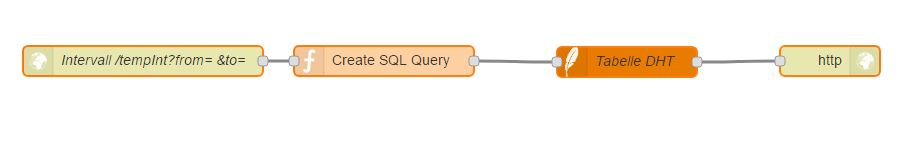
\includegraphics[scale=0.7]{images/tempIntFlow}
	\caption{Beispiel: Temperatur Intervall abfragen}
	\label{flow:TempInt}
\end{figure}
Damit der User nicht nur basierend auf der Rule Engine Sensordaten geliefert bekommt, wird über Node Red eine \acf{API} erstellt, die jederzeit angesprochen werden kann um die neusten Daten anzuzeigen. Die \ac{URL} setzt sich aus der \ac{IP}-Adresse des Raspberry's dem Port 1880 für Node-Red und einen relative Pfad zusammen. 
\\Die \ac{API} hat folgenden Schnittstellen, die über \ac{HTTP}-Get Request angesprochen werden können:
\begin{itemize}
	\item \textbf{/temp}: Diese Route liefert dem User den aktuellen, vom Temperatur- \& Luftfeuchtigkeitssensor gemessenen Wert zurück. 
	\item \textbf{/tempInt}: Um sich den Temperaturverlauf innerhalb eines begrenzten Zeitraums sich anzeigen zu lassen, kann diese Route angesprochen werden. Dabei müssen an den relativen Pfad zwei Parameter, \enqoute{from} und \enqoute{to},  gesetzt werden.  Beiden Parametern muss ein Datum in der Form \enquote{dd.mm.yyyy} übergeben werden. \\Die Anfrage setzt sich dann aus der \ac{IP}-Adresse, dem Port, sowie dem relativen Pfad zusammen und hat beispielsweise folgende Form: \enquote{192.168.0.100:1880/temInt?from=10.05.2017\&to=25.05.2017}
	\item \textbf{/window}:
	\item \textbf{/picture}:
	\item \textbf{/motion}:
	\item \textbf{/mqgas}:
	\item \textbf{/gasInt}:
	\item \textbf{/temp}:
\end{itemize}

Außerdem werden noch Flows benötigt, die innerhalb eines definierten Intervalls die aktuellen Sensordaten abfragen und anschließen in der entsprechenden Datenbanktabelle abspeichern. In ABBILDUNG XX ist beispielhaft aufgezeigt, wie der Datenfluss in Node-Red modelliert ist, damit alle 5 Minuten ein Datenbankeintrag erstellt wird. 




\section{Grafische Benutzeroberfläche} %Louisa
Als grafische Benutzerschnittstelle für das in dieser Arbeit erläuterte System wird eine ortsunabhängige Lösung entwickelt (F-10.2). Um eine Ortsunabhängigkeit gewährleisten zu können, bietet es sich an ein mobiles Endgerät zu entwickeln. Es wurde  entschieden als Benutzerschnittstelle eine Android App zu nutzen, aus dem Grund, dass Android den höchsten Endkundenabsatz besitzt \cite{statista:marktanteileandroid} und dadurch eine größere Maße erreicht werden kann.
\subsection{Rule Engine}
Die Rule Engine wird nach den Anforderungen aus Kapitel \ref{sec:Anforderungen} entwickelt. Demnach muss die Rule Engine dem Nutzer ermöglichen dynamisch Regeln hinzufügen zu können oder wieder zu löschen (F-30.1). Grenzwerte oder Wertebereiche kann der Nutzer für die erfassten Datentypen (F-10) selbst bestimmen (F-30.2). Des Weiteren soll die Rule Engine zeitliche Aspekte in den Regeldefinitionen einbinden können. Der Nutzer kann demnach zeitliche Intervalle festlegen, in denen ein Wert oder Wertebereich gehalten werden soll. Die Definition von Datenabhängikeiten kann von der Rule Engine verarbeitet werden, um optimalere Aktionen auslösen zu können (F-30.5).\\
Es werden mögliche Rule Engines recherchiert, die die gestellten Anforderungen erfüllen. Dabei wurden nur Rule Engines betrachtet, die in Android genutzt werden können, sowie welche mit regelmäßigen Releases. Aus der Recherche haben sich folgende Rule Engine Bibliotheken ergeben:
\begin{itemize}
	\item Easy Rules \cite{github:easyrules}
	\item OpenRules \cite{openrules}
	\item RuleBook \cite{github:rulebook}
\end{itemize}
Diese Rule Engines bieten gute Möglichkeiten Regeln zu erstellen und diese zu überprüfen. Der entscheidende gemeinsame Nachteil dieser Rule Engines ist die Implementierung der Regeln. Durch die Recherche konnte keine Engine gefunden werden, die eine dynamische Erstellung von neuen Regeln über die Oberfläche ermöglichen. Die Definition neuer Regeln durch den Nutzer ohne den Quellcode zu veränder ist jedoch eine essentielle Anforderung. Aus diesem Grund wurde sich dafür entschieden, eine Rule Engine selbst zu implementieren.\\
Bei der Implementierung der Rule Engine wurden die Ergebnisse der Recherche miteinbezogen. Vor allem an die Struktur der Regeln zu ihren Wenn- und Dann-Teilen der Regel Engine RuleBook wurde bei der Implementierung betrachtet.


- Warum keine RuleEngine Bibliothek nutzen?
-mögliche Rule Engines: es wurden nur RuleEngines betrachtet, die in Android genutzt werden können
- Easy Rules
- OpenRules
- Dredd
- RuleBook
-Vorteile:  
- Nachteile bzw. Vorteile von diesen Engines
- Warum keine bekannt Rule Sprache nutzen um Regeln zu definieren? - RuleML

\subsection{Daten Anzeige}